% ============================================================
%  GAN Body Lab — Memoria del Proyecto
%  Redes Neuronales y Aprendizaje Profundo · RNAP UA
%  Universidad de Alicante · Ingeniería en Inteligencia Artificial
% ============================================================
\documentclass[a4paper,11pt]{article}

% --- Codificación y lengua ---
\usepackage[utf8]{inputenc}
\usepackage[T1]{fontenc}
\usepackage[spanish,es-nodecimaldot]{babel}

% --- Geometría y tipografía ---
\usepackage[top=2.5cm, bottom=2.5cm, left=2.8cm, right=2.8cm]{geometry}
\usepackage{lmodern}
\usepackage{microtype}
\usepackage{setspace}
\onehalfspacing

% --- Matemáticas ---
\usepackage{amsmath, amssymb, amsthm}
\usepackage{mathtools}
\usepackage{bm}

% --- Figuras y tablas ---
\usepackage{graphicx}
\usepackage{float}
\usepackage{caption}
\usepackage{subcaption}
\usepackage{booktabs}
\usepackage{array}
\usepackage{multirow}
\usepackage{tabularx}

% --- Código fuente ---
\usepackage{listings}
\usepackage{xcolor}

\definecolor{codegreen}{rgb}{0,0.6,0}
\definecolor{codegray}{rgb}{0.5,0.5,0.5}
\definecolor{codepurple}{rgb}{0.58,0,0.82}
\definecolor{backcolour}{rgb}{0.97,0.97,0.97}
\definecolor{keyblue}{rgb}{0.0,0.3,0.7}

\lstdefinestyle{mystyle}{
    backgroundcolor=\color{backcolour},
    commentstyle=\color{codegreen},
    keywordstyle=\color{keyblue}\bfseries,
    numberstyle=\tiny\color{codegray},
    stringstyle=\color{codepurple},
    basicstyle=\ttfamily\footnotesize,
    breakatwhitespace=false,
    breaklines=true,
    captionpos=b,
    keepspaces=true,
    numbers=left,
    numbersep=5pt,
    showspaces=false,
    showstringspaces=false,
    showtabs=false,
    tabsize=2,
    frame=single,
    rulecolor=\color{gray!40},
}
\lstset{style=mystyle}

% --- Algoritmos ---
\usepackage{algorithm}
\usepackage{algpseudocode}
\algrenewcommand\algorithmicforall{\textbf{for each}}

% --- Hipervínculos ---
\usepackage[hidelinks, colorlinks=true,
            linkcolor=blue!60!black,
            citecolor=green!50!black,
            urlcolor=blue!70!black]{hyperref}

% --- Encabezados y pie de página ---
\usepackage{fancyhdr}
\pagestyle{fancy}
\fancyhf{}
\fancyhead[L]{\small\textit{GAN Body Lab}}
\fancyhead[R]{\small\textit{RNAP UA · 2026}}
\fancyfoot[C]{\thepage}
\renewcommand{\headrulewidth}{0.4pt}

% --- Miscelánea ---
\usepackage{enumitem}
\usepackage{csquotes}
\usepackage{tcolorbox}
\tcbuselibrary{most}

% --- Bibliografía ---
\usepackage[style=numeric, sorting=none, backend=biber]{biblatex}
\addbibresource{main.bib}

% ============================================================
%  DOCUMENTO
% ============================================================
\begin{document}

% ---- Portada -----------------------------------------------
\begin{titlepage}
    \centering
    \vspace*{1.5cm}
    {\Huge\bfseries GAN Body Lab\par}
    \vspace{0.5cm}
    {\Large Generación de Cuerpos Humanos mediante\\
    Redes Generativas Adversariales\par}
    \vspace{2cm}
    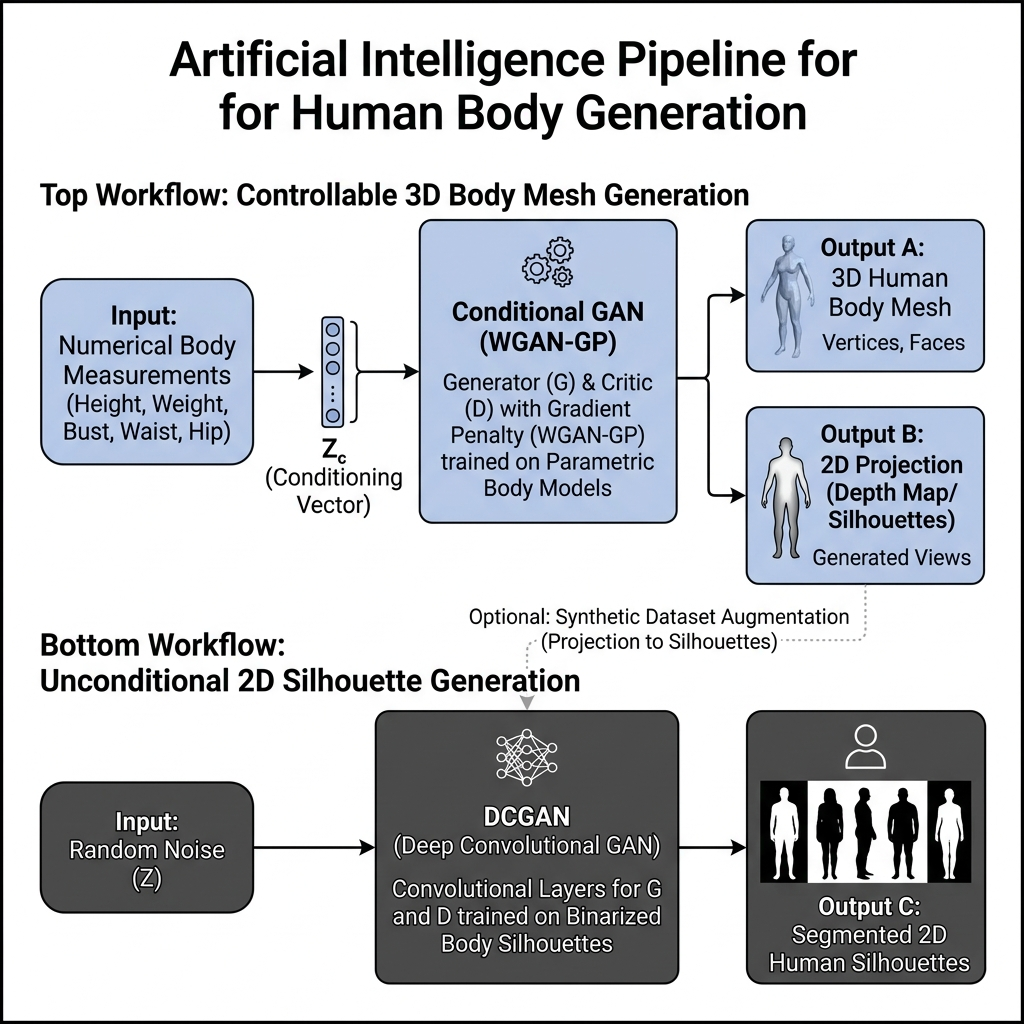
\includegraphics[width=0.55\textwidth]{../docs/readme/pipeline.png}
    \vspace{2cm}

    \begin{tabular}{ll}
        \textbf{Autores:} &
        Santiago Álvarez Geanta \\
        & Alejandro García Belmonte \\
        & Guillermo García Blázquez \\
        & Taron Sargsyan \\[8pt]
        \textbf{Asignatura:} & Redes Neuronales y Aprendizaje Profundo \\
        \textbf{Institución:} & Universidad de Alicante ·
                                Ingeniería en Inteligencia Artificial \\
        \textbf{Fecha:}       & Mayo 2026 \\
    \end{tabular}

    \vfill
    {\small
        \href{mailto:sag82@alu.ua.es}{sag82@alu.ua.es}
    }
\end{titlepage}

% ---- Índice ------------------------------------------------
\tableofcontents
\newpage

% ============================================================
\section{Introducción y Motivación}
% ============================================================

El presente proyecto, denominado \textbf{GAN Body Lab}, aborda el problema
de la generación sintética de cuerpos humanos a partir de datos
antropométricos. Esta tarea tiene aplicaciones directas en industrias como
la moda, el diseño ergonómico, la medicina y los videojuegos, donde disponer
de avatares corporales realistas y controlables supone una ventaja
significativa.

La motivación central surge de una pregunta práctica: ¿es posible construir
un modelo que, recibiendo únicamente un conjunto reducido de medidas corporales
(altura, contorno de pecho, cintura, cadera, etc.), sea capaz de sintetizar
una forma corporal 3D plausible y coherente con esas restricciones? La respuesta
que este proyecto propone es afirmativa, y se apoya en el uso de
\textbf{Redes Generativas Adversariales} (GANs) condicionadas por las medidas
de entrada.

El proyecto implementa tres pipelines complementarios e independientes:

\begin{enumerate}[leftmargin=*, label=(\arabic*)]
    \item \textbf{Pipeline Tabular (MLP)}: aprende una correspondencia generativa entre
          medidas antropométricas y parámetros de forma del modelo SMPL
          (\textit{betas}). La salida puede exportarse como imagen 2D (PNG) o
          malla 3D (OBJ).
    \item \textbf{Pipeline de Imagen}: aprende la distribución visual de imágenes
          de cuerpos humanos segmentados del dataset TNT15, generando siluetas
          plausibles desde ruido aleatorio, sin condicionamiento explícito.
    \item \textbf{Pipeline Tab Transformer}: una rama experimental que explora
          el uso de un Transformer sobre nubes de puntos 3D como condición,
          sirviendo de línea base negativa para demostrar que la representación
          del condicionamiento importa tanto como la arquitectura.
\end{enumerate}

Los tres pipelines comparten la misma arquitectura de pérdida,
\textbf{WGAN-GP} (Wasserstein GAN con Gradient Penalty)~\cite{gulrajani2017},
que es una de las variantes más estables del framework GAN original propuesto
por Goodfellow et al.\ en 2014~\cite{goodfellow2014}.

% ============================================================
\section{Fundamentos Teóricos de las GANs}
% ============================================================

\subsection{Contexto: Modelos Generativos}

Los modelos generativos aprenden a estimar la distribución subyacente $p(\bm{x})$
de los datos de entrenamiento con el fin de generar nuevas muestras realistas.
Los tres paradigmas principales son:

\begin{description}[leftmargin=!, labelwidth=2.5cm]
    \item[\textbf{VAE}] Codifica datos en un espacio latente estructurado y los
          reconstruye. Entrenamiento estable, pero produce muestras desenfocadas.
    \item[\textbf{GAN}] Enfrenta un generador contra un discriminador en un juego
          adversarial. Alta calidad visual, pero inestable y propenso al
          \textit{mode collapse}.
    \item[\textbf{Diffusion}] Revierte un proceso gradual de adición de ruido.
          Máxima calidad y diversidad, pero inferencia lenta (muchos pasos de
          denoising).
\end{description}

El presente proyecto opta por GANs porque las salidas de alta nitidez son
prioritarias, y la comunidad ha desarrollado variantes estables (WGAN-GP)
que hacen el entrenamiento manejable.

\subsection{El Framework GAN Original}
\label{sec:gan_original}

Las Redes Generativas Adversariales fueron introducidas por
Goodfellow et al.~\cite{goodfellow2014} en el artículo seminal
\textit{``Generative Adversarial Nets''} (NIPS 2014). El framework propone
entrenar simultáneamente dos redes:

\begin{itemize}
    \item \textbf{Generador $G$}: aprende una distribución $p_g$ sobre los datos.
          Recibe ruido latente $\bm{z} \sim p_z(\bm{z})$ y lo mapea al espacio
          de datos mediante $G(\bm{z};\,\theta_g)$. Su objetivo es que sus
          muestras sean indistinguibles de los datos reales.
    \item \textbf{Discriminador $D$}: recibe muestras reales
          $\bm{x} \sim p_{\text{data}}(\bm{x})$ y falsas $G(\bm{z})$, y produce
          un escalar $D(\bm{x};\,\theta_d)$ que estima la probabilidad de que
          $\bm{x}$ provenga de los datos reales. Su objetivo es clasificar
          correctamente reales de falsos.
\end{itemize}

La metáfora de los autores es ilustrativa: $G$ actúa como falsificadores
que producen moneda falsa, mientras que $D$ actúa como la policía que intenta
detectarlos. La competición entre ambos los impulsa a mejorar mutuamente.

\subsection{La Función Objetivo Minimax}

El entrenamiento conjunto de $G$ y $D$ corresponde a un juego minimax de dos
jugadores con la función de valor $V(G,D)$:

\begin{equation}
    \label{eq:minimax}
    \min_{G}\;\max_{D}\;V(D,G)
    = \mathbb{E}_{\bm{x}\sim p_{\text{data}}(\bm{x})}\!\left[\log D(\bm{x})\right]
    + \mathbb{E}_{\bm{z}\sim p_z(\bm{z})}\!\left[\log\!\left(1-D(G(\bm{z}))\right)\right]
\end{equation}

\paragraph{Interpretación de cada término.}

\begin{itemize}
    \item $\mathbb{E}\!\left[\log D(\bm{x})\right]$: $D$ recibe una muestra
          \emph{real} $\bm{x}$ y quiere que $D(\bm{x})\to 1$, es decir,
          $\log D(\bm{x})\to 0$ (máximo). Si $D$ es engañado y produce 0.5,
          entonces $\log(0.5)=-0.69$, lo cual es peor para él.
    \item $\mathbb{E}\!\left[\log(1-D(G(\bm{z})))\right]$: $G$ genera una muestra
          falsa. $D$ quiere $D(G(\bm{z}))\to 0$; $G$ quiere lo contrario:
          $D(G(\bm{z}))\to 1$, haciendo este término muy negativo (mínimo).
\end{itemize}

En la práctica, $\log(1-D(G(\bm{z})))$ satura cuando $D$ rechaza
confiadamente las muestras al inicio. Por eso, en la práctica se entrena $G$
para \emph{maximizar} $\log D(G(\bm{z}))$: el punto fijo es el mismo,
pero los gradientes son más fuertes al inicio.

\subsection{La Distribución Normal como Espacio Latente}

El ruido latente $\bm{z}$ se muestrea de $\mathcal{N}(\bm{0},\bm{I})$.
Esta elección no es arbitraria:

\begin{itemize}
    \item La distribución normal cubre todo $\mathbb{R}^n$ sin ``zonas muertas'',
          eliminando regiones del espacio latente que nunca se explorarían.
    \item Cualquier distribución puede obtenerse transformando una normal
          mediante una función suficientemente expresiva (y una red profunda
          lo es).
    \item $\mathcal{N}(\bm{0},\bm{I})$ es \emph{isotrópica}: todas las
          direcciones latentes son tratadas por igual, lo que hace funcionar
          la interpolación y la aritmética de vectores en el espacio latente.
\end{itemize}

En el presente proyecto, el generador tabular usa $\text{noise\_dim}=64$ y
el generador de imagen usa $\text{noise\_dim}=128$.

\subsection{El Equilibrio de Nash y la Convergencia}

Desde la teoría de juegos, el entrenamiento busca el \textbf{equilibrio de Nash}:
ningún jugador puede mejorar cambiando únicamente su propia estrategia.
Esto ocurre cuando $D(G(\bm{z}))=0.5$: el discriminador esencialmente lanza
una moneda, porque las muestras falsas son indistinguibles de las reales.

Goodfellow et al.\ demostraron formalmente:

\begin{tcolorbox}[colback=blue!5!white, colframe=blue!50!black, title=Proposición 1 (Discriminador Óptimo)]
Para $G$ fijo, el discriminador óptimo $D^*$ es:
\begin{equation}
    \label{eq:dstar}
    D^*_G(\bm{x}) = \frac{p_{\text{data}}(\bm{x})}{p_{\text{data}}(\bm{x}) + p_g(\bm{x})}
\end{equation}
\end{tcolorbox}

\begin{tcolorbox}[colback=green!5!white, colframe=green!50!black, title=Teorema 1 (Óptimo Global)]
El mínimo global del criterio de entrenamiento $C(G)$ se alcanza si y solo si
$p_g = p_{\text{data}}$. En ese punto, $C(G) = -\log 4$.
\end{tcolorbox}

La función de valor del minimax puede reformularse en términos de la
\textbf{divergencia Jensen-Shannon}:

\begin{equation}
    \label{eq:jsd}
    C(G) = -\log 4 + 2\cdot\text{JSD}(p_{\text{data}} \,\|\, p_g)
\end{equation}

Dado que JSD es siempre no-negativa y vale cero solo cuando las distribuciones
son iguales, el único mínimo global es $p_g = p_{\text{data}}$.

\begin{figure}[H]
    \centering
    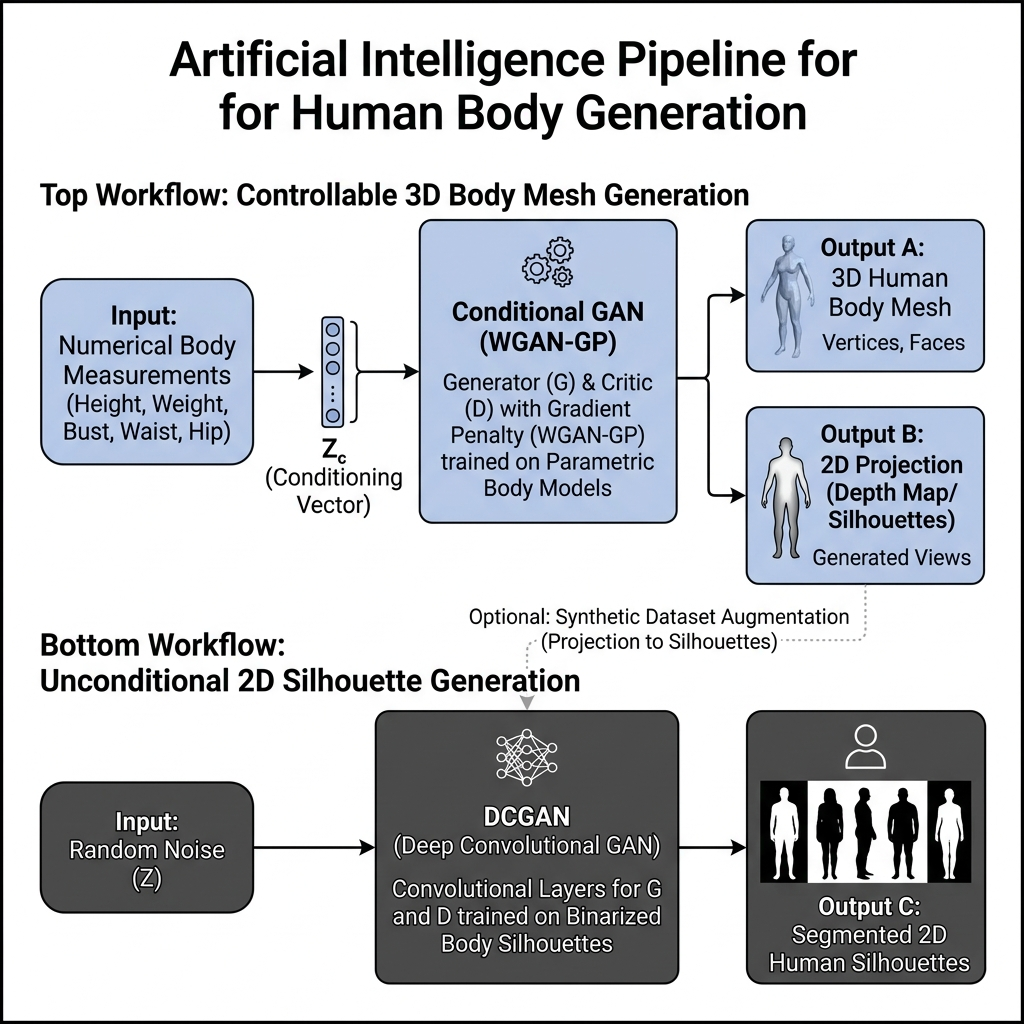
\includegraphics[width=0.85\textwidth]{../docs/readme/pipeline.png}
    \caption{Pipeline completo del sistema GAN Body Lab. \textbf{Arriba:}
    workflow de generación de malla 3D condicionada por medidas (Conditional
    WGAN-GP + SMPL). \textbf{Abajo:} workflow de generación de siluetas 2D
    incondicional (DCGAN + WGAN-GP sobre TNT15).}
    \label{fig:pipeline}
\end{figure}

\subsection{Algoritmo de Entrenamiento}

El Algoritmo~\ref{alg:gan} es el algoritmo de entrenamiento minimax por
lotes estocásticos presentado en el paper original.

\begin{algorithm}[H]
\caption{Entrenamiento minibatch estocástico de GANs (Goodfellow et al., 2014)}
\label{alg:gan}
\begin{algorithmic}[1]
\For{número de iteraciones de entrenamiento}
    \For{$k$ pasos}
        \State Muestrear $\{\bm{z}^{(1)},\ldots,\bm{z}^{(m)}\} \sim p_z(\bm{z})$
        \State Muestrear $\{\bm{x}^{(1)},\ldots,\bm{x}^{(m)}\} \sim p_{\text{data}}(\bm{x})$
        \State Actualizar $D$ ascendiendo su gradiente estocástico:
        \[
            \nabla_{\theta_d}\;\frac{1}{m}\sum_{i=1}^{m}
            \Bigl[\log D\!\left(\bm{x}^{(i)}\right)
            +\log\!\left(1-D\!\left(G\!\left(\bm{z}^{(i)}\right)\right)\right)\Bigr]
        \]
    \EndFor
    \State Muestrear $\{\bm{z}^{(1)},\ldots,\bm{z}^{(m)}\} \sim p_z(\bm{z})$
    \State Actualizar $G$ descendiendo su gradiente estocástico:
    \[
        \nabla_{\theta_g}\;\frac{1}{m}\sum_{i=1}^{m}
        \log\!\left(1-D\!\left(G\!\left(\bm{z}^{(i)}\right)\right)\right)
    \]
\EndFor
\end{algorithmic}
\end{algorithm}

% ============================================================
\section{Variantes y Mejoras de las GANs}
% ============================================================

\subsection{DCGAN: Deep Convolutional GAN}

Propuesto por Radford et al.~\cite{radford2015}, DCGAN introduce las siguientes
guías de arquitectura para GANs convolucionales estables:

\begin{itemize}
    \item Reemplazar el \textit{pooling} con convoluciones con \textit{stride}
          (discriminador) y convoluciones fraccionadas (\textit{generator}).
    \item Usar \textit{BatchNorm} tanto en el generador como en el discriminador.
    \item Eliminar las capas completamente conectadas en arquitecturas profundas.
    \item Usar \texttt{ReLU} en el generador (excepto la salida, que usa
          \texttt{Tanh}).
    \item Usar \texttt{LeakyReLU} en el discriminador en todas las capas.
\end{itemize}

\subsection{Conditional GAN (cGAN)}
\label{sec:cgan}

Propuesta por Mirza y Osindero~\cite{mirza2014} en
\textit{``Conditional Generative Adversarial Nets''} (2014), la cGAN extiende
el framework GAN añadiendo información de condicionamiento $\bm{y}$ a ambas
redes. La función objetivo condicionada es:

\begin{equation}
    \label{eq:cgan}
    \min_{G}\;\max_{D}\;V(D,G)
    = \mathbb{E}_{\bm{x}\sim p_{\text{data}}(\bm{x})}\!\left[\log D(\bm{x}\mid\bm{y})\right]
    + \mathbb{E}_{\bm{z}\sim p_z(\bm{z})}\!\left[\log\!\left(1-D(G(\bm{z}\mid\bm{y}))\right)\right]
\end{equation}

En el generador, el ruido $p_z(\bm{z})$ y $\bm{y}$ se combinan en una
representación oculta conjunta. En el discriminador, $\bm{x}$ e $\bm{y}$
se presentan como entradas adicionales. En el presente proyecto, el Generador
tabular es exactamente una cGAN: recibe tanto $\bm{z}\in\mathbb{R}^{64}$
como las 10 medidas corporales normalizadas, y genera los 10 parámetros
$\bm{\beta}$ SMPL condicionados a esas medidas.

\subsection{WGAN y WGAN-GP}

\subsubsection{Problemas del GAN original}

El GAN original sufre dos problemas principales:

\begin{enumerate}
    \item \textbf{Gradientes desaparecidos}: cuando $D$ es demasiado bueno al
          inicio, $\log(1-D(G(\bm{z})))\approx 0$ y el gradiente del generador
          se desvanece.
    \item \textbf{Mode collapse}: $G$ aprende a producir siempre el mismo output,
          ignorando la diversidad real del espacio de datos.
\end{enumerate}

\subsubsection{WGAN-GP (Gulrajani et al., 2017)}

WGAN-GP~\cite{gulrajani2017} reemplaza la función de valor por la distancia
de Wasserstein e impone la restricción 1-Lipschitz mediante una
\textbf{penalización del gradiente}:

\begin{equation}
    \label{eq:wgangp_loss}
    \mathcal{L}_D =
    -\,\mathbb{E}\!\left[D(\bm{x}_{\text{real}})\right]
    +\,\mathbb{E}\!\left[D(G(\bm{z}))\right]
    +\;\lambda\;\mathbb{E}\!\left[\!\left(\left\|\nabla_{\hat{\bm{x}}}\,
    D(\hat{\bm{x}})\right\|_2 - 1\right)^2\right]
\end{equation}

\begin{equation}
    \label{eq:wgangp_g}
    \mathcal{L}_G = -\,\mathbb{E}\!\left[D(G(\bm{z}))\right]
\end{equation}

donde $\hat{\bm{x}} = \alpha\,\bm{x}_{\text{real}} + (1-\alpha)\,G(\bm{z})$,
con $\alpha\sim\mathcal{U}[0,1]$, y $\lambda=10$ (usado en este proyecto
como \texttt{lambda\_gp=10.0}).

\begin{tcolorbox}[colback=orange!5!white, colframe=orange!60!black,
                  title=Nota técnica: BatchNorm $\times$ WGAN-GP]
La penalización del gradiente requiere derivar la salida del discriminador
respecto a cada muestra individualmente. BatchNorm acopla las muestras del
batch, lo que rompe ese supuesto. Por eso, en todos los discriminadores de este
proyecto se usa \textbf{GroupNorm(num\_groups=1)} o \textbf{LayerNorm}
(equivalentes cuando se normaliza por muestra) en lugar de BatchNorm.
\end{tcolorbox}

% ============================================================
\section{Descripción del Proyecto}
% ============================================================

\subsection{Objetivos}

\begin{enumerate}
    \item Implementar una Conditional WGAN-GP que mapee 10 medidas
          antropométricas a 10 parámetros de forma SMPL ($\bm{\beta}$).
    \item Implementar un sistema de ajuste de $\bm{\beta}$ SMPL
          (pseudo-ground-truth) mediante optimización Gauss-Newton no lineal.
    \item Implementar un DCGAN + WGAN-GP capaz de generar siluetas humanas
          plausibles desde ruido aleatorio usando TNT15.
    \item Implementar un Tab Transformer condicionado por nubes de puntos
          3D como línea base experimental, y evaluar con métricas
          generativas (FID e Inception Score).
    \item Proveer una CLI completa (\texttt{main.py}) para entrenar, evaluar
          e inferir con los tres pipelines.
\end{enumerate}

\subsection{Pipeline General}

El sistema completo, ilustrado en la Figura~\ref{fig:pipeline}, se divide en
tres workflows:

\begin{description}
    \item[\textbf{Workflow 1 — MLP tabular}] (Generación de malla 3D controlable):
          Recibe medidas numéricas corporales combinadas con un vector de
          condicionamiento $Z_c$. Entra en una Conditional WGAN-GP y produce
          dos salidas: (A) malla 3D del cuerpo humano (vértices/caras, OBJ)
          y (B) proyección 2D (mapa de profundidad/siluetas, PNG).
    \item[\textbf{Workflow 2 — DCGAN de imagen}] (Generación incondicional de siluetas 2D):
          Recibe ruido aleatorio $Z$ que entra en una DCGAN entrenada sobre
          siluetas binarizadas del dataset TNT15, produciendo siluetas 2D
          segmentadas.
    \item[\textbf{Workflow 3 — Tab Transformer}] (Línea base experimental):
          Recibe una nube de 256 puntos 3D submuestreados de SMPL junto con
          ruido latente $Z$. Un Transformer procesa los tokens geométricos
          y genera los 10 parámetros $\bm{\beta}$ SMPL. Sirve para comparar
          el efecto de la representación del condicionamiento frente al MLP.
\end{description}

% ============================================================
\section{Datasets}
% ============================================================

\subsection{NOMO3D: Medidas Antropométricas}

NOMO3D es el dataset principal del pipeline tabular. Contiene medidas corporales
de sujetos humanos reales en formato textual (ficheros \texttt{.txt} con líneas
\texttt{MEASURE nombre=valor} en centímetros). El sistema lee 10 medidas para
construir el vector de condicionamiento:

\begin{table}[H]
    \centering
    \caption{Medidas corporales usadas como vector de condicionamiento.}
    \label{tab:medidas}
    \begin{tabular}{@{}ll@{}}
        \toprule
        \textbf{Campo NOMO3D} & \textbf{Significado físico} \\
        \midrule
        \texttt{Head\_Top\_Height}        & Altura total del cuerpo (cm)          \\
        \texttt{BUST\_Circ}               & Contorno de pecho/busto (cm)          \\
        \texttt{NaturalWAIST\_Circ}       & Contorno de cintura natural (cm)      \\
        \texttt{HIP\_Circ}                & Contorno de cadera (cm)               \\
        \texttt{NeckBase\_Circ}           & Contorno de cuello en la base (cm)    \\
        \texttt{Shoulder\_to\_Shoulder}   & Anchura de hombros (cm)               \\
        \texttt{Inseam}                   & Tiro interior (cm)                    \\
        \texttt{Outseam}                  & Largo exterior de pierna (cm)         \\
        \texttt{Thigh\_Circ}              & Contorno de muslo (cm)                \\
        \texttt{Bicep\_Circ}              & Contorno de bíceps (cm)               \\
        \bottomrule
    \end{tabular}
\end{table}

La división train/test es 80\%/20\% (configurable), con semilla fija
(\texttt{np.random.seed(42)}) para reproducibilidad. Las medidas se normalizan
con Z-score calculado sobre el conjunto de entrenamiento y guardado en
\texttt{internal/experiments/meas\_scaler.npz}.

\subsection{SMPL: Modelo Paramétrico de Cuerpo Humano}

SMPL~\cite{loper2015} (Skinned Multi-Person Linear Model) es el modelo
paramétrico de cuerpo humano que sirve de ``capa de decodificación'' para
convertir los $\bm{\beta}$ generados por la GAN en una malla 3D coherente.
SMPL describe la forma corporal mediante:

\begin{itemize}
    \item \textbf{Parámetros de forma $\bm{\beta} \in \mathbb{R}^{10}$}: captura
          variaciones de forma entre individuos (talla, complexión, proporciones).
    \item \textbf{Parámetros de pose $\bm{\theta}$}: ángulos articulares.
    \item La malla resultante tiene \textbf{6890 vértices} y $\approx$13000 caras.
\end{itemize}

\subsection{TNT15: Dataset de Siluetas}

TNT15 contiene cuatro sujetos (\texttt{mr}, \texttt{pz}, \texttt{sg},
\texttt{sp}) grabados desde cinco cámaras (\texttt{00}–\texttt{04}), con
PNGs ya segmentados (sujeto en gris sobre fondo negro).

\begin{itemize}
    \item $\approx$100\,000 frames brutos; $\approx$20\,600 efectivos tras
          submuestreo con \texttt{frame\_stride=5}.
    \item Imágenes en escala de grises (1 canal).
    \item Redimensionado a $64\times64$, normalización a $[-1,1]$.
    \item Split train/test: 90\%/10\% por orden alfabético.
\end{itemize}

% ============================================================
\section{Arquitectura del Sistema}
% ============================================================

\subsection{Pipeline Tabular MLP: Medidas $\to$ Cuerpo SMPL}

El pipeline tabular es una Conditional GAN donde generador y discriminador
son MLP:

\begin{align*}
    \text{Entradas del generador:}\quad   & \bm{z}\in\mathbb{R}^{64},\quad
                                             \bm{c}\in\mathbb{R}^{10} \text{ (medidas norm.)} \\
    \text{Salida del generador:}\quad      & \bm{\beta}\in\mathbb{R}^{10} \text{ (shape params SMPL)} \\
    \text{Entradas del discriminador:}\quad & \bm{\beta}\in\mathbb{R}^{10},\quad
                                              \bm{c}\in\mathbb{R}^{10} \\
    \text{Salida del discriminador:}\quad  & s\in\mathbb{R} \text{ (score Wasserstein, sin activación)}
\end{align*}

\subsection{Pipeline de Imagen: Ruido $\to$ Silueta Humana}

El pipeline de imagen sigue DCGAN + WGAN-GP sin condicionamiento:

\begin{align*}
    \text{Entrada del generador:}\quad   & \bm{z}\in\mathbb{R}^{128} \\
    \text{Salida del generador:}\quad    & \bm{I}\in\mathbb{R}^{1\times64\times64}
                                           \text{ (imagen en } [-1,1]) \\
    \text{Entrada del discriminador:}\quad & \bm{I}\in\mathbb{R}^{1\times64\times64} \\
    \text{Salida del discriminador:}\quad  & s\in\mathbb{R} \text{ (sin sigmoid)}
\end{align*}

\subsection{Pipeline Tab Transformer: Nube de Puntos $\to$ Cuerpo SMPL}

El pipeline Tab Transformer es una Conditional GAN donde generador y
discriminador son Transformers que procesan nubes de puntos 3D como tokens:

\begin{align*}
    \text{Entradas del generador:}\quad   & \bm{z}\in\mathbb{R}^{64},\quad
                                             \bm{P}\in\mathbb{R}^{256\times3} \text{ (nube de puntos norm.)} \\
    \text{Salida del generador:}\quad      & \bm{\beta}\in\mathbb{R}^{10} \text{ (shape params SMPL)} \\
    \text{Entradas del discriminador:}\quad & \bm{\beta}\in\mathbb{R}^{10},\quad
                                              \bm{P}\in\mathbb{R}^{256\times3} \\
    \text{Salida del discriminador:}\quad  & s\in\mathbb{R} \text{ (score Wasserstein, sin activación)}
\end{align*}

La arquitectura detallada de este pipeline se describe en la
Sección~\ref{sec:tab_transformer}.

% ============================================================
\section{Modelos Implementados}
% ============================================================

\subsection{Generador Tabular Condicional}

\textbf{Archivo:} \texttt{src/models/generator.py}

El generador implementado es \texttt{\_GeneratorWithResidual}, que divide
la red en tres segmentos:

\paragraph{Pre-peak.} Desde la entrada concatenada
$[\bm{z};\bm{c}]\in\mathbb{R}^{74}$ hasta el pico de dimensionalidad:

\begin{center}
\texttt{Linear(74$\to$256) + LayerNorm + LeakyReLU(0.2)} \\
\texttt{Linear(256$\to$512) + LayerNorm + LeakyReLU(0.2)} \\
\texttt{Linear(512$\to$1024) + LayerNorm + LeakyReLU(0.2)}
\end{center}

\paragraph{Bloque residual} en el pico ($\text{dim}=1024$):
\[
    \text{ResBlock}(\bm{x}) = \text{LeakyReLU}\!\left(\bm{x}
    + \bigl[\text{Lin}\to\text{LN}\to\text{LReLU}\to\text{Lin}\to\text{LN}\bigr](\bm{x})\right)
\]

\paragraph{Post-peak} hasta la salida:
\begin{center}
\texttt{Linear(1024$\to$512) + LayerNorm + LeakyReLU(0.2)} \\
\texttt{Linear(512$\to$256) + LayerNorm + LeakyReLU(0.2)} \\
\texttt{Linear(256$\to$10)} \hspace{0.5em} \textit{(sin activación)}
\end{center}

Inicialización: Kaiming Normal con $a=0.2$; sesgo=0.

\subsection{Discriminador Tabular}

\textbf{Archivo:} \texttt{src/models/discriminator.py}

\begin{center}
$[\bm{\beta};\bm{c}]\in\mathbb{R}^{20}$
$\xrightarrow{\text{Lin}+\text{LReLU}}$ 256
$\xrightarrow{\text{Lin}+\text{LReLU}}$ 128
$\xrightarrow{\text{Lin}+\text{LReLU}}$ 64
$\xrightarrow{\text{Lin}}$ $\mathbb{R}$ (sin sigmoid)
\end{center}

Sin BatchNorm: la penalización del gradiente WGAN-GP requiere independencia
entre muestras, que BatchNorm viola.

\subsection{Generador de Imagen (DCGAN)}

\textbf{Archivo:} \texttt{src/models/img\_generator.py}

Arquitectura para $64\times64$, 1 canal, \texttt{noise\_dim}=128,
\texttt{g\_feature\_maps}=64:

\begin{table}[H]
    \centering
    \caption{Arquitectura del ImgGenerator.}
    \label{tab:imggen}
    \begin{tabular}{@{}llll@{}}
        \toprule
        \textbf{Capa} & \textbf{Operación} & \textbf{Tamaño salida} & \textbf{Norm.} \\
        \midrule
        Entrada       & reshape            & $(B,128,1,1)$          & —              \\
        ConvT1        & $4\times4$, s=1    & $(B,512,4,4)$          & BN + ReLU      \\
        ConvT2        & $4\times4$, s=2    & $(B,256,8,8)$          & BN + ReLU      \\
        ConvT3        & $4\times4$, s=2    & $(B,128,16,16)$        & BN + ReLU      \\
        ConvT4        & $4\times4$, s=2    & $(B,64,32,32)$         & BN + ReLU      \\
        ConvT5 (out)  & $4\times4$, s=2    & $(B,1,64,64)$          & Tanh           \\
        \bottomrule
    \end{tabular}
\end{table}

El número de bloques se calcula automáticamente como
$n = \log_2(\texttt{image\_size})-2$, haciendo la arquitectura
independiente del tamaño objetivo.

\subsection{Discriminador de Imagen (Crítico CNN)}

\textbf{Archivo:} \texttt{src/models/img\_discriminator.py}

\begin{table}[H]
    \centering
    \caption{Arquitectura del ImgDiscriminator.}
    \label{tab:imgdisc}
    \begin{tabular}{@{}llll@{}}
        \toprule
        \textbf{Capa} & \textbf{Operación} & \textbf{Tamaño salida} & \textbf{Norm.} \\
        \midrule
        Entrada       & —                  & $(B,1,64,64)$          & —              \\
        Conv1         & $4\times4$, s=2    & $(B,64,32,32)$         & LeakyReLU      \\
        Conv2         & $4\times4$, s=2    & $(B,128,16,16)$        & GN(1)+LReLU    \\
        Conv3         & $4\times4$, s=2    & $(B,256,8,8)$          & GN(1)+LReLU    \\
        Conv4         & $4\times4$, s=2    & $(B,512,4,4)$          & GN(1)+LReLU    \\
        Conv5 (out)   & $4\times4$, s=1    & $(B,1,1,1)$            & —              \\
        flatten       & —                  & $(B,1)$                & sin sigmoid    \\
        \bottomrule
    \end{tabular}
\end{table}

\texttt{GroupNorm(num\_groups=1)}: equivalente a LayerNorm sobre $(C,H,W)$.
Normaliza por muestra de forma independiente, respetando el supuesto de
independencia requerido por WGAN-GP.

% ============================================================
\section{Pre-procesamiento: Beta Fitter (Gauss-Newton)}
% ============================================================

\textbf{Archivo:} \texttt{src/data/beta\_fitter.py}

Antes de entrenar la GAN tabular, se obtiene para cada muestra de NOMO3D
el vector $\bm{\beta}^*$ que mejor reproduce las 10 medidas del dataset.
La cadena de medición (MeasureBody sobre trimesh) no es diferenciable, por
lo que se usa diferencias finitas centrales para el Jacobiano.

\begin{algorithm}[H]
\caption{Ajuste de $\bm{\beta}$ SMPL por Gauss-Newton}
\label{alg:gn}
\begin{algorithmic}[1]
\Require{Target de medidas $\bm{t}\in\mathbb{R}^{10}$, género, tolerancias}
\Ensure{$\bm{\beta}^*\in[-3,3]^{10}$}

\State \textbf{Fase 1 — Warm-start lineal (linearización en $\bm{\beta}=\bm{0}$):}
\State $\bm{m}_0 \gets \text{SMPL}(\bm{0},\text{gender})$
\For{$k = 0,\ldots,9$}
    \State $J_{:,k} \gets [\text{SMPL}(\bm{0}+\varepsilon\bm{e}_k) - \text{SMPL}(\bm{0}-\varepsilon\bm{e}_k)] / (2\varepsilon)$
\EndFor
\State $\bm{\beta}_0 \gets \text{clip}(\text{lstsq}(J,\, \bm{t}-\bm{m}_0),\,-3,3)$

\State \textbf{Fase 2 — Gauss-Newton iterativo (re-linearización en $\bm{\beta}_k$):}
\For{$\text{iter} = 1,\ldots,8$}
    \State Re-computar $J_k$ en $\bm{\beta}_k$ (idem, costo $2\cdot10+1$ eval.)
    \State $\Delta\bm{\beta} \gets \text{lstsq}(J_k,\;\bm{t}-\text{SMPL}(\bm{\beta}_k))$
    \State Backtracking: halvar \textit{step} hasta $\|r_{\text{trial}}\| \le \|r_k\|$
    \State $\bm{\beta}_{k+1} \gets \text{clip}(\bm{\beta}_k + \text{step}\cdot\Delta\bm{\beta},\,-3,3)$
    \If{$\|\Delta\bm{\beta}\| < 10^{-3}$ o mejora relativa $< 10^{-4}$}
        \State \textbf{break}
    \EndIf
\EndFor
\State \Return $\bm{\beta}_k$
\end{algorithmic}
\end{algorithm}

Los $\bm{\beta}$ ajustados se guardan en
\texttt{internal/data/betas\_cache/\{id\}.npy}; las estadísticas de
convergencia en \texttt{internal/logs/beta\_fit\_stats.csv}.

% ============================================================
\section{Entrenamiento WGAN-GP}
% ============================================================

\subsection{Hiperparámetros}

\begin{table}[H]
    \centering
    \caption{Hiperparámetros de entrenamiento para ambos pipelines.}
    \label{tab:hparams}
    \begin{tabularx}{\textwidth}{lXX}
        \toprule
        \textbf{Hiperparámetro} & \textbf{Tabular (HParams)} & \textbf{Imagen (ImgHParams)} \\
        \midrule
        \texttt{noise\_dim}      & 64               & 128 \\
        \texttt{batch\_size}     & 128              & 64  \\
        \texttt{epochs}          & 3\,000           & 100 \\
        \texttt{lr\_g = lr\_d}   & $10^{-4}$        & $10^{-4}$ \\
        $\beta_1,\,\beta_2$      & 0.5,\;0.9        & 0.5,\;0.9 \\
        \texttt{n\_critic}       & 5                & 5   \\
        \texttt{lambda\_gp}      & 10.0             & 10.0 \\
        \texttt{g\_hidden\_dims} & [256,512,1024,512,256] & — \\
        \texttt{image\_size}     & —                & 64  \\
        \texttt{channels}        & —                & 1 (grayscale) \\
        \texttt{frame\_stride}   & —                & 5   \\
        \texttt{train\_split}    & 0.8              & 0.9 \\
        \bottomrule
    \end{tabularx}
\end{table}

\paragraph{Justificación de $\beta_1=0.5$, $\beta_2=0.9$.}
Los valores por defecto de Adam ($0.9$, $0.999$) introducen demasiada inercia
para WGAN-GP. Con $\beta_1=0.5$ se reduce el momentum y el entrenamiento
es más estable, tal como recomienda el paper de Gulrajani.

\paragraph{Justificación de \texttt{n\_critic=5}.}
El discriminador se actualiza 5 veces por cada actualización del generador.
Esto da al crítico tiempo de adaptarse antes de que $G$ se mueva, lo que
es crucial para que la estimación de la distancia de Wasserstein sea fiable.

\subsection{Loop de Entrenamiento Tabular}

Por cada batch $(\bm{c}, \bm{\beta}_{\text{real}})$ del dataset NOMO3D:

\begin{lstlisting}[language=Python, caption={Loop WGAN-GP tabular (extracto de train.py)}]
# Normalizar medidas
meas_norm = (meas - meas_mean) / meas_std

# --- n_critic=5 pasos del Discriminador ---
for _ in range(n_critic):
    z = torch.randn(batch, noise_dim)
    beta_fake = G(z, meas_norm).detach()
    d_real = D(beta_real, meas_norm)
    d_fake = D(beta_fake, meas_norm)
    gp = compute_gradient_penalty(beta_real, beta_fake, meas_norm)
    L_D = -d_real.mean() + d_fake.mean() + lambda_gp * gp
    L_D.backward(); opt_D.step()

# --- 1 paso del Generador ---
z = torch.randn(batch, noise_dim)
beta_fake = G(z, meas_norm)
L_G = -D(beta_fake, meas_norm).mean()
L_G.backward(); opt_G.step()
\end{lstlisting}

\subsection{Gradient Penalty: Implementación}

\begin{lstlisting}[language=Python, caption={compute\_gradient\_penalty (train.py)}]
def compute_gradient_penalty(real, fake, cond):
    # Interpolar entre muestras reales y falsas
    alpha = torch.rand(real.size(0), 1, device=device)
    x_hat = (alpha * real + (1-alpha) * fake).requires_grad_(True)
    d_hat = D(x_hat, cond)
    # Calcular gradiente respecto a la interpolacion
    grads = autograd.grad(outputs=d_hat, inputs=x_hat,
                          grad_outputs=torch.ones_like(d_hat),
                          create_graph=True)[0]
    grads = grads.view(grads.size(0), -1)
    gp = ((grads.norm(2, dim=1) - 1) ** 2).mean()
    return gp
\end{lstlisting}

Para el discriminador de imagen, \texttt{alpha} tiene forma
$(B,1,1,1)$ en lugar de $(B,1)$, para interpolar en el espacio de imagen
$\mathbb{R}^{1\times64\times64}$.

% ============================================================
\section{Inferencia y Resultados}
% ============================================================

\subsection{Inferencia Tabular (2D y 3D)}

El proceso de inferencia tabular sigue estos pasos:

\begin{enumerate}
    \item Cargar el último checkpoint \texttt{wgangp\_ckpt\_*.pt} (por mtime).
    \item Cargar el scaler (\texttt{meas\_scaler.npz}) del entrenamiento.
    \item Normalizar las 10 medidas de entrada.
    \item Generar $N=32$ muestras $\bm{z}\sim\mathcal{N}(\bm{0},\bm{I})$ en paralelo.
    \item Pasar todas por $G$ y promediar: $\bm{\beta}^* = \frac{1}{N}\sum_{i=1}^{N}G(\bm{z}_i,\bm{c})$.
    \item Instanciar SMPL con $\bm{\beta}^*$ y el género → vértices + caras.
    \item Exportar como PNG (render ortográfico 2D) y/o OBJ (malla 3D).
\end{enumerate}

La estrategia de promediar $N=32$ muestras reduce la varianza de muestreo
del espacio latente, dando una estimación más estable y representativa de la
forma corporal condicionada a las medidas dadas.

\begin{figure}[H]
    \centering
    \begin{subfigure}[b]{0.38\textwidth}
        \centering
        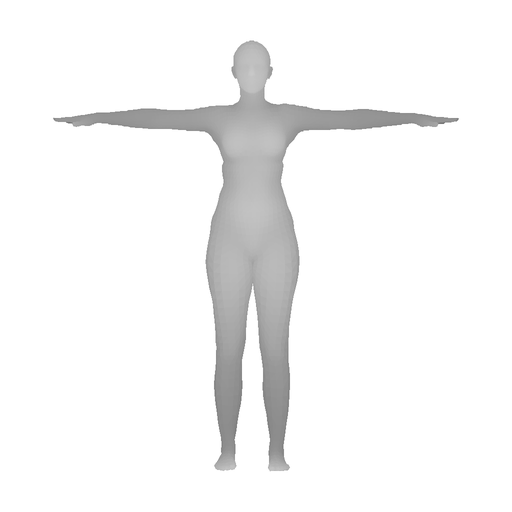
\includegraphics[width=\textwidth]{../docs/readme/output_2d.png}
        \caption{Salida 2D: proyección ortográfica del cuerpo generado
        (vista frontal, femenino, 170 cm).}
        \label{fig:out2d}
    \end{subfigure}
    \hfill
    \begin{subfigure}[b]{0.56\textwidth}
        \centering
        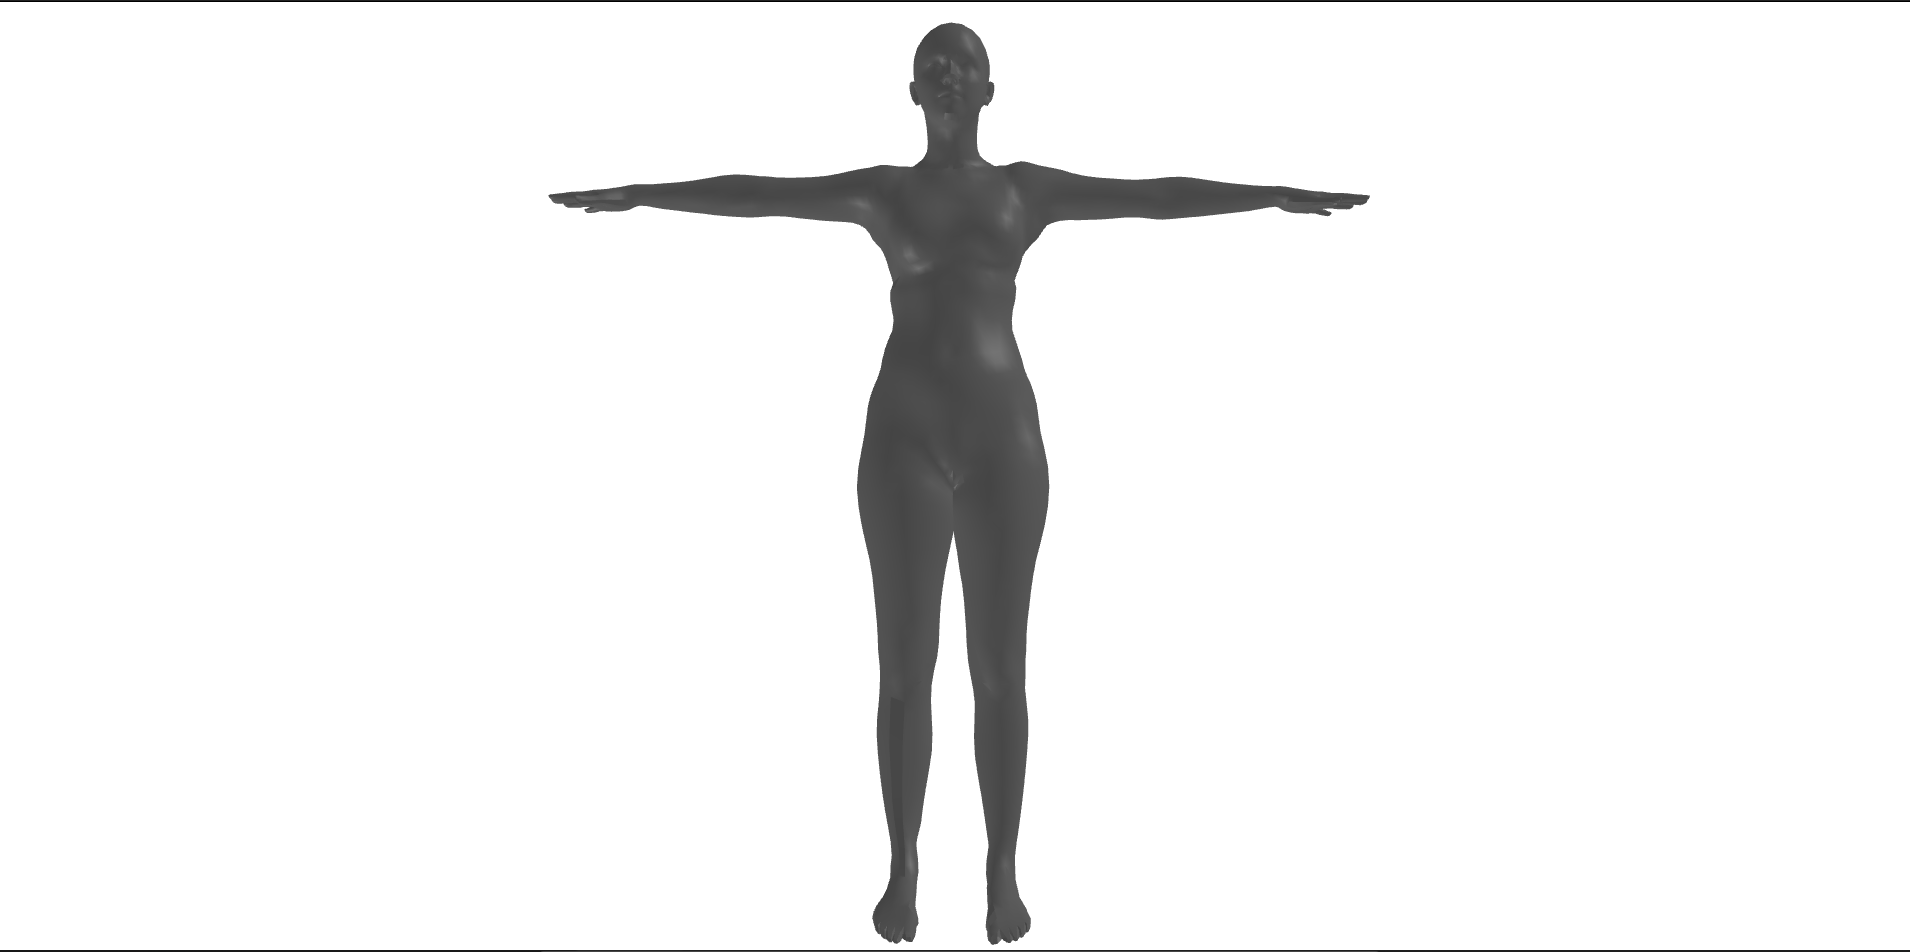
\includegraphics[width=\textwidth]{../docs/readme/output_3d.png}
        \caption{Salida 3D: malla SMPL de 6890 vértices renderizada por el
        visor de trimesh.}
        \label{fig:out3d}
    \end{subfigure}
    \caption{Resultados del pipeline tabular (Conditional WGAN-GP + SMPL).
    Las proporciones corporales (cintura, cadera, hombros) reflejan el vector
    de medidas introducido como condición.}
    \label{fig:outputs}
\end{figure}

\subsection{Salida 2D — Proyección Ortográfica}

La Figura~\ref{fig:out2d} muestra un cuerpo femenino en pose-T (pose canónica
de SMPL), vista frontal. El render 2D es un proyector ortográfico ligero
(\texttt{src/render\_2d.py}) que no requiere OpenGL ni ventana, haciéndolo
portátil para servidores de entrenamiento.

\subsection{Salida 3D — Malla SMPL}

La Figura~\ref{fig:out3d} muestra la malla 3D con sus 6890 vértices. Se
observan las proporciones características del vector $\bm{\beta}$ generado
por la GAN, que es diferente para cada combinación de medidas de entrada.

\subsection{Grid de Imágenes TNT15}

\begin{figure}[H]
    \centering
    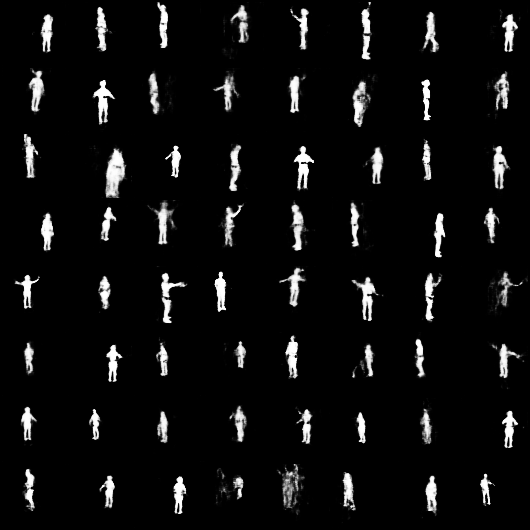
\includegraphics[width=0.75\textwidth]{../docs/readme/image_gan_grid.png}
    \caption{Grid $8\times8$ de 64 siluetas generadas por el ImgGenerator
    (DCGAN + WGAN-GP) entrenado sobre TNT15. Se observa diversidad de poses,
    proporciones corporales y orientaciones.}
    \label{fig:imagegrid}
\end{figure}

La Figura~\ref{fig:imagegrid} muestra el resultado del pipeline de imagen.
Las siluetas presentan diversidad en posturas (brazos en distintos ángulos),
proporciones y orientaciones, lo que indica que el modelo ha aprendido la
distribución de poses del dataset TNT15 (personas en movimiento).

% ============================================================
\section{Evaluación de los Modelos}
% ============================================================

\subsection{Evaluación del Pipeline MLP Tabular (MAE)}

\textbf{Archivo:} \texttt{src/eval.py}

La evaluación del modelo MLP tabular usa el \textbf{Error Absoluto Medio}
(MAE) en centímetros, calculado comparando las medidas del cuerpo generado
por SMPL con las medidas target del split de test:

\begin{equation}
    \label{eq:mae}
    \text{MAE}(m) = \frac{1}{N_{\text{test}}}\sum_{i=1}^{N_{\text{test}}}
    \left|\hat{m}_i - m_i^*\right| \quad [\text{cm}]
\end{equation}

donde $\hat{m}_i$ es la medida del cuerpo generado por SMPL para la muestra
$i$ del test, y $m_i^*$ es la medida target de NOMO3D.

El proceso es:
\begin{enumerate}
    \item Para cada muestra del test, generar $\bm{\beta}$ con la GAN condicionada.
    \item Instanciar SMPL y medir el cuerpo generado.
    \item Calcular el MAE por medida y promediar sobre el test.
\end{enumerate}

El resultado es una tabla con MAE por dimensión que permite identificar qué
medidas aprende mejor el modelo a reproducir.

\subsection{Evaluación del Tab Transformer (FID e IS)}

La evaluación del pipeline Tab Transformer utiliza métricas generativas
(FID e Inception Score) en lugar del MAE, ya que su condición de entrada
no son medidas sino nubes de puntos. Los detalles de estas métricas y sus
resultados se presentan en la Sección~\ref{sec:tab_transformer}.

% ============================================================
\section{Reflexión: Estabilidad y Modos de Fallo}
% ============================================================

\subsection{Mode Collapse}

El mode collapse es el principal riesgo del entrenamiento GAN: el generador
aprende a producir siempre el mismo output. En el pipeline tabular, se
manifestaría como que $G$ genera siempre los mismos 10 $\bm{\beta}$ sin
importar las medidas de condicionamiento.

WGAN-GP mitiga este problema porque la distancia de Wasserstein proporciona
gradientes útiles incluso cuando las distribuciones no se solapan. La
penalización del gradiente asegura que el crítico sea 1-Lipschitz, lo que
estabiliza el entrenamiento.

\subsection{Gradientes Desaparecidos}

El uso de \texttt{LeakyReLU} (slope=0.2 en la parte negativa) evita la
``muerte'' de neuronas durante el entrenamiento adversarial. El bloque
residual en el generador tabular proporciona una conexión directa que
preserva el flujo de gradientes.

\subsection{Normalización de Medidas}

Las 10 medidas tienen escalas muy diferentes (altura $\approx170$ cm,
bíceps $\approx28$ cm). Sin normalizar, la altura dominaría la pérdida.
La normalización Z-score transforma las medidas a $\mathcal{N}(0,1)$,
equiparando el peso de cada dimensión.

% ============================================================
\section{Estructura del Repositorio}
% ============================================================

\begin{lstlisting}[language=bash, caption={Estructura del repositorio.}]
.
|-- main.py                  # CLI (fit/train/eval/infer/train_img/infer_img
|                            #       train_tab/eval_tab/infer_tab)
|-- requirements.txt
|-- src/
|   |-- config/              # hparams.py, paths.py
|   |-- data/                # dataset.py, img_dataset.py, pc_dataset.py,
|   |                        #   beta_fitter.py
|   |-- models/              # generator, discriminator, img_generator,
|   |                        #   img_discriminator, tab_generator,
|   |                        #   tab_discriminator
|   |-- smpl_module_project/ # measure, evaluate, landmark/joint/measurement defs
|   |-- train.py             # WGANGPTrainer (tabular MLP)
|   |-- train_img.py         # ImgWGANGPTrainer (imagen)
|   |-- train_tab.py         # TabWGANGPTrainer (Tab Transformer)
|   |-- inference.py         # Inferencia tabular -> 2D/3D
|   |-- inference_img.py     # Inferencia imagen -> PNG/grid
|   |-- infer_tab.py         # Inferencia Tab Transformer -> 2D/3D
|   |-- eval.py              # MAE sobre split de test (MLP)
|   |-- eval_tab.py          # FID + IS comparativa (MLP vs Tab Transformer)
|   `-- render_2d.py         # Proyector ortografico 2D
|-- docs/readme/             # pipeline.png, output_2d.png, output_3d.png,
|                            #   image_gan_grid.png
|-- laTex/                   # Memoria en LaTeX
|-- notebooks/               # pipeline_completo.ipynb
`-- internal/                # [NO versionado] datos, checkpoints, logs, salidas
\end{lstlisting}

% ============================================================
\section{Pipeline Tab Transformer: Nubes de Puntos $\to$ Cuerpo SMPL}
\label{sec:tab_transformer}
% ============================================================

Además de los dos pipelines anteriores (tabular MLP y DCGAN de imagen), el
proyecto implementa una \textbf{tercera rama experimental} basada en un
\textbf{Tab Transformer}~\cite{huang2020} condicionado por \emph{nubes de
puntos 3D} extraídas del modelo SMPL. El objetivo de esta rama no es superar
al MLP condicionado por medidas antropométricas, sino servir como
\textbf{línea base negativa} que demuestre empíricamente que la
\emph{representación del condicionamiento} importa tanto o más que la
complejidad de la arquitectura.

\subsection{Motivación: ¿Por qué un Transformer sobre nubes de puntos?}

La hipótesis que motiva este experimento es la siguiente: el Tab Transformer
fue diseñado por Huang et al.\ para datos tabulares, donde cada
\emph{feature} (columna de una tabla) se trata como un token independiente y
se procesa mediante \emph{self-attention}. En nuestro caso, se aplica
\textbf{deliberadamente} esta arquitectura a un dominio para el que no fue
concebida: cada punto 3D $(x,y,z)$ del cuerpo se trata como si fuera una
columna tabular, sin codificación posicional geométrica, sin invarianza a
rotación ni a escala, y sin noción explícita de vecindad espacial.

El resultado esperado es que el Transformer tendrá que ``redescubrir'' las
relaciones geométricas del cuerpo humano exclusivamente a partir de la
señal de entrenamiento, algo que arquitecturas especializadas en nubes de
puntos como PointNet~\cite{qi2017} o DGCNN~\cite{wang2019} codifican de
forma nativa. Si el Tab Transformer obtiene peores resultados que el MLP
condicionado por medidas, quedará demostrado que una representación compacta
y bien diseñada (10 medidas antropométricas) es más eficaz que una
representación de alta dimensionalidad (256 puntos $\times$ 3 coordenadas
= 768 dimensiones) procesada por una arquitectura inadecuada.

\subsection{Dataset de Nubes de Puntos}

\textbf{Archivo:} \texttt{src/data/pc\_dataset.py}

El dataset de nubes de puntos reutiliza los vectores $\bm{\beta}$
pseudo-ground-truth obtenidos previamente por el ajuste Gauss-Newton
(Algoritmo~\ref{alg:gn}), almacenados en
\texttt{internal/data/betas\_cache/*.npy}. Para cada muestra, la generación
de la nube de puntos sigue los pasos:

\begin{enumerate}
    \item \textbf{Carga del modelo SMPL sin chumpy}: el archivo
          \texttt{SMPL\_FEMALE.pkl} (o \texttt{MALE}) se carga con
          \texttt{pickle}. Dado que los \texttt{.pkl} originales del proyecto
          SMPL contienen objetos \texttt{chumpy.Ch}, el cargador inyecta un
          módulo \emph{stub} de chumpy en \texttt{sys.modules} que convierte
          automáticamente los arrays de chumpy a arrays NumPy estándar. Tras
          la carga, los stubs se eliminan de \texttt{sys.modules}. Esta
          técnica evita instalar chumpy, que tiene incompatibilidades con
          NumPy $\geq$ 1.24 y Python $\geq$ 3.11.

    \item \textbf{Cómputo de vértices}: la forma del cuerpo se calcula
          mediante la formulación lineal de SMPL:
          \begin{equation}
              \label{eq:smpl_shape}
              \bm{V} = \bm{T} + \sum_{k=0}^{9}\beta_k\,\bm{S}_k
          \end{equation}
          donde $\bm{T}\in\mathbb{R}^{6890\times3}$ es el \emph{template}
          (forma media), $\bm{S}_k\in\mathbb{R}^{6890\times3}$ es la $k$-ésima
          dirección principal de deformación (\texttt{shapedirs}), y $\beta_k$
          son los parámetros de forma. El resultado es una malla de
          \textbf{6\,890 vértices} $\times$ 3 coordenadas.

    \item \textbf{Submuestreo}: de los 6\,890 vértices, se seleccionan
          $N_p = 256$ (configurable vía \texttt{TabHParams.n\_pc\_points})
          usando una semilla fija (\texttt{np.random.seed(0)}). Los índices
          resultantes se \emph{ordenan} para estabilidad numérica y se
          reutilizan de forma determinista en entrenamiento, evaluación e
          inferencia. La nube de puntos resultante tiene forma
          $(256,\,3)$.

    \item \textbf{Caché}: cada nube generada se guarda en
          \texttt{internal/data/pc\_cache/\{id\}.npy} para evitar recomputarla
          en cada epoch. El coste de la primera generación es despreciable
          ($\approx$\,2~ms por muestra), pero el caché elimina la latencia
          de I/O del \texttt{.pkl} SMPL en epochs sucesivos.
\end{enumerate}

El split train/test utiliza la \textbf{misma semilla y la misma proporción
80\%/20\%} que el \texttt{NOMODataset} tabular, garantizando que las mismas
muestras van al conjunto de test en ambas ramas y que la comparación de
métricas es justa.

\subsubsection{Normalización de las nubes de puntos}

Las coordenadas $(x,y,z)$ de los vértices SMPL están en metros y tienen
escalas y offsets muy diferentes por eje (por ejemplo, la coordenada $y$
es predominantemente positiva, con rango $\approx[0,\,1.8]$, mientras que
$x$ y $z$ oscilan simétricamente alrededor de cero). Sin normalizar, las
activaciones del Transformer estarían sesgadas y el aprendizaje sería
ineficiente.

Se aplica una \textbf{normalización Z-score por eje}, calculada sobre
\emph{todos los puntos del split de entrenamiento}:
\begin{equation}
    \hat{p}_{ij} = \frac{p_{ij} - \mu_j}{\sigma_j}, \quad j \in \{x,y,z\}
\end{equation}
donde $\mu_j$ y $\sigma_j$ son la media y desviación típica del eje $j$
sobre el conjunto de entrenamiento. Las estadísticas se guardan en
\texttt{internal/experiments/pc\_scaler.npz} y se reutilizan durante la
evaluación y la inferencia, de forma análoga al \texttt{meas\_scaler.npz}
del pipeline MLP.

\subsection{Generador Tab Transformer}

\textbf{Archivo:} \texttt{src/models/tab\_generator.py}

El generador recibe dos entradas: un vector de ruido
$\bm{z}\in\mathbb{R}^{64}$ y una nube de puntos
$\bm{P}\in\mathbb{R}^{256\times3}$ (condición). El flujo de datos se
descompone en cinco etapas:

\begin{enumerate}
    \item \textbf{Embedding de puntos}: cada punto 3D $(x,y,z)$ se proyecta
          a un token de dimensión $d=64$ mediante:
          \[
            \texttt{Linear}(3 \to 64) \;\to\; \texttt{LayerNorm}(64)
            \;\to\; \texttt{LeakyReLU}(0.2)
          \]
          Esto produce una secuencia de 256 tokens de dimensión 64:
          $\bm{T}_p \in \mathbb{R}^{B \times 256 \times 64}$.

    \item \textbf{Inyección de ruido}: el vector $\bm{z}$ se proyecta
          a $256 \times 64 = 16\,384$ dimensiones y se remodela a
          $(B, 256, 64)$:
          \[
            \texttt{Linear}(64 \to 16384) \;\to\; \texttt{LayerNorm}
            \;\to\; \texttt{LeakyReLU}(0.2) \;\to\; \texttt{reshape}
          \]
          Los tokens de ruido se \textbf{suman} (no concatenan) a los tokens
          de punto: $\bm{T} = \bm{T}_p + \bm{T}_z$. La suma mantiene la
          dimensión constante y actúa como una perturbación estocástica sobre
          la representación geométrica, inyectando diversidad sin duplicar
          el número de tokens.

    \item \textbf{Encoding posicional aprendible}: se suma un tensor
          $\bm{E} \in \mathbb{R}^{1 \times 256 \times 64}$, inicializado
          con $\mathcal{N}(0, 0.02)$, que permite al Transformer distinguir
          la posición ordinal de cada punto en la secuencia.

    \item \textbf{Transformer Encoder}: 3 capas de
          \texttt{TransformerEncoderLayer} con los siguientes hiperparámetros:

          \begin{table}[H]
              \centering
              \caption{Configuración del Transformer Encoder
                       (generador Tab Transformer).}
              \label{tab:tabgen_transformer}
              \begin{tabular}{@{}ll@{}}
                  \toprule
                  \textbf{Parámetro} & \textbf{Valor} \\
                  \midrule
                  \texttt{d\_model}         & 64 \\
                  \texttt{nhead}            & 4 (dim por cabeza = 16) \\
                  \texttt{num\_layers}      & 3 \\
                  \texttt{dim\_feedforward}  & 128 \\
                  Activación               & GELU \\
                  Dropout                  & 0.1 \\
                  Normalización            & pre-layer (\texttt{norm\_first=True}) \\
                  \texttt{batch\_first}     & True \\
                  \bottomrule
              \end{tabular}
          \end{table}

          Cada capa aplica \emph{self-attention} sobre los 256 tokens,
          permitiendo que cada punto ``vea'' la geometría global del
          cuerpo a través de las puntuaciones de atención.

    \item \textbf{Cabeza de salida}: \emph{mean-pooling} sobre la dimensión
          temporal de los 256 tokens, seguido de:
          \[
            \texttt{LayerNorm}(64) \;\to\; \texttt{Linear}(64 \to 10)
          \]
          El vector resultante $\bm{\beta} \in \mathbb{R}^{10}$ son los
          parámetros de forma SMPL predichos, \textbf{sin activación final}
          (los betas SMPL pueden tomar valores en $\mathbb{R}$, aunque en
          la práctica se limitan al rango $[-3, 3]$).
\end{enumerate}

La inicialización de pesos usa \textbf{Kaiming Normal} con pendiente
$a=0.2$ (consistente con LeakyReLU) y sesgo inicializado a cero. El número
total de parámetros es del orden de $\sim$150\,K, significativamente menor
que el generador MLP ($\sim$1.5\,M) gracias a la reutilización de pesos
en las capas de atención.

\subsection{Discriminador Tab Transformer}

\textbf{Archivo:} \texttt{src/models/tab\_discriminator.py}

El discriminador recibe los betas (reales o generados) junto con la nube
de puntos condicionante, y produce un escalar (sin sigmoid, por ser WGAN).
Su arquitectura presenta una diferencia conceptual clave respecto al
generador: los betas se tratan como \textbf{tokens individuales con
embeddings separados por posición}.

\begin{enumerate}
    \item \textbf{Embedding de betas}: cada uno de los 10 parámetros
          $\beta_k$ se trata como un token independiente con su propia
          capa de proyección:
          \[
            \beta_k \in \mathbb{R}
            \;\xrightarrow{\text{Lin}_k(1 \to 64)}\;
            \texttt{LayerNorm}(64)
            \;\to\; \texttt{LeakyReLU}(0.2)
          \]
          Usar una \texttt{ModuleList} de 10 capas \emph{independientes}
          (en lugar de una capa compartida) es el rasgo distintivo del
          Tab Transformer frente a un embedding compartido: cada ``columna''
          ($\beta_0, \beta_1, \ldots, \beta_9$) aprende su propia
          representación, capturando la semántica diferente de cada
          componente principal de deformación SMPL.

    \item \textbf{Embedding de puntos}: igual que en el generador,
          cada punto 3D se proyecta a un token de dimensión 64 mediante
          una capa \texttt{Linear(3, 64)} compartida.

    \item \textbf{Concatenación}: los 10 tokens de beta y los 256 tokens
          de punto se concatenan en una secuencia de \textbf{266 tokens}
          de dimensión 64:
          $\bm{T} \in \mathbb{R}^{B \times 266 \times 64}$.

    \item \textbf{Encoding posicional + Transformer}: mismo esquema que el
          generador (3 capas, 4 cabezas, GELU, pre-norm), pero con una
          secuencia de 266 tokens en lugar de 256.

    \item \textbf{Cabeza de salida}: mean-pool sobre los 266 tokens,
          seguido de $\texttt{LayerNorm}(64) \to \texttt{Linear}(64 \to 1)$.
\end{enumerate}

\begin{tcolorbox}[colback=orange!5!white, colframe=orange!60!black,
                  title=Nota técnica: ausencia de BatchNorm]
El discriminador Tab Transformer \textbf{no usa BatchNorm en ningún punto},
por las mismas razones que el discriminador de imagen (§6.4): el gradient
penalty de WGAN-GP requiere independencia entre muestras del batch para
calcular correctamente $\|\nabla_{\hat{\bm{x}}} D(\hat{\bm{x}})\|_2$.
BatchNorm acopla las estadísticas del batch, violando este supuesto. Las
capas \texttt{LayerNorm} integradas en los bloques Transformer y en los
embeddings normalizan por muestra individual, respetando la independencia.
\end{tcolorbox}

\subsection{Hiperparámetros del Tab Transformer}

\begin{table}[H]
    \centering
    \caption{Hiperparámetros de entrenamiento del pipeline Tab Transformer,
             comparados con el pipeline MLP tabular.}
    \label{tab:tab_hparams}
    \begin{tabularx}{\textwidth}{lXX}
        \toprule
        \textbf{Hiperparámetro} & \textbf{MLP (HParams)} & \textbf{Tab Transformer (TabHParams)} \\
        \midrule
        \texttt{noise\_dim}      & 64              & 64 \\
        Condición de entrada     & 10 medidas (cm) & 256 puntos 3D \\
        \texttt{batch\_size}     & 128             & 32 \\
        \texttt{epochs}          & 3\,000          & 3\,000 \\
        \texttt{lr\_g = lr\_d}   & $10^{-4}$       & $10^{-4}$ \\
        $\beta_1,\,\beta_2$      & 0.5,\;0.9       & 0.5,\;0.9 \\
        \texttt{n\_critic}       & 5               & 5 \\
        \texttt{lambda\_gp}      & 10.0            & 10.0 \\
        \texttt{d\_model}        & —               & 64 \\
        \texttt{nhead}           & —               & 4 \\
        \texttt{num\_layers}     & —               & 3 \\
        \texttt{dim\_feedforward} & —              & 128 \\
        \texttt{n\_pc\_points}   & —               & 256 \\
        \texttt{train\_split}    & 0.8             & 0.8 \\
        Prefijo de checkpoint    & \texttt{wgangp\_ckpt\_*} & \texttt{wgangp\_tab\_ckpt\_*} \\
        \bottomrule
    \end{tabularx}
\end{table}

\paragraph{Justificación de \texttt{batch\_size=32}.}
El batch size del Tab Transformer (32) es cuatro veces menor que el del MLP
(128). Esto se debe al mayor coste por muestra del mecanismo de self-attention:
con 256 tokens, la complejidad de la atención es $\mathcal{O}(N^2 \cdot d)
= \mathcal{O}(256^2 \cdot 64) \approx 4.2\,\text{M}$ operaciones por capa
por muestra, frente a las $\sim$500\,K operaciones del forward MLP. Un batch
mayor agotaría la memoria GPU o ralentizaría excesivamente cada iteración.

\subsection{Bucle de Entrenamiento}

\textbf{Archivo:} \texttt{src/train\_tab.py}

El trainer \texttt{TabWGANGPTrainer} sigue el patrón WGAN-GP ya establecido
en los otros pipelines, con tres particularidades relevantes:

\paragraph{Gradient penalty condicionado.}
La interpolación $\alpha \sim \mathcal{U}[0,1]$ se aplica \textbf{únicamente
sobre los betas}, no sobre la nube de puntos (que es la condición fija):
\begin{equation}
    \hat{\bm{\beta}} = \alpha\,\bm{\beta}_{\text{real}}
    + (1-\alpha)\,\bm{\beta}_{\text{fake}},
    \qquad \alpha \sim \mathcal{U}[0,1]
\end{equation}
El discriminador recibe $(\hat{\bm{\beta}},\,\bm{P})$ y los gradientes se
toman respecto a $\hat{\bm{\beta}}$ solamente. Esta formulación es coherente
con la definición de WGAN-GP: el crítico debe ser Lipschitz respecto a los
\emph{datos} ($\bm{\beta}$), no respecto a la \emph{condición} ($\bm{P}$).

\paragraph{Normalización on-the-fly.}
Cada batch de nubes de puntos se normaliza usando $\mu_j$ y $\sigma_j$
calculados al inicio del entrenamiento sobre todo el split de training.

\paragraph{Log de muestras generadas.}
Cada 100 epochs, se genera un vector de betas usando la primera nube de
puntos del training set (\texttt{\_probe\_pc}) con ruido aleatorio fresco,
y se escribe en un CSV (\texttt{internal/logs/tab\_beta\_samples.csv}).
Esto permite trazar la evolución temporal de los betas generados y
detectar posibles colapsos de modos durante el entrenamiento.

\subsection{Evaluación: FID e Inception Score Tabulares}

\textbf{Archivo:} \texttt{src/eval\_tab.py}

La evaluación del Tab Transformer emplea dos métricas generativas
adaptadas al dominio tabular, que permiten comparar cuantitativamente
la calidad y diversidad de los betas generados.

\subsubsection{FID Tabular (Fréchet Inception Distance)}

En el contexto de generación de imágenes, el FID se calcula sobre
\emph{features} extraídas por una red InceptionV3 pre-entrenada. En nuestro
caso, los ``datos'' ya son vectores de baja dimensión
($\bm{\beta}\in\mathbb{R}^{10}$), por lo que el FID se calcula
\textbf{directamente sobre los vectores de betas}, sin necesidad de un
extractor de features intermedio.

Se modelan las distribuciones de betas reales y generados como
gaussianas multivariantes $\mathcal{N}(\bm{\mu}_r, \bm{\Sigma}_r)$ y
$\mathcal{N}(\bm{\mu}_g, \bm{\Sigma}_g)$, y se aplica la fórmula de la
distancia de Fréchet:

\begin{equation}
    \label{eq:fid}
    \text{FID} = \|\bm{\mu}_r - \bm{\mu}_g\|^2_2
    + \text{Tr}\!\left(\bm{\Sigma}_r + \bm{\Sigma}_g
    - 2\left(\bm{\Sigma}_r\,\bm{\Sigma}_g\right)^{1/2}\right)
\end{equation}

La raíz cuadrada de la matriz $\bm{\Sigma}_r\,\bm{\Sigma}_g$ se calcula
mediante \texttt{scipy.linalg.sqrtm}, con eliminación de la parte
imaginaria residual para estabilidad numérica. Un \textbf{FID bajo}
indica que la distribución generada se asemeja a la distribución real.
Para datos de 10 dimensiones, valores por debajo de $\sim$10 se
consideran buenos; por encima de 50, la discrepancia es significativa.

\subsubsection{Inception Score Tabular}

El Inception Score (IS) mide simultáneamente la \emph{calidad} (cada muestra
se clasifica con alta confianza) y la \emph{diversidad} (las muestras se
reparten entre muchas clases) de las muestras generadas. En generación de
imágenes, se usa un clasificador InceptionV3 pre-entrenado; en nuestro
dominio tabular, \textbf{no existe tal clasificador}, por lo que se entrena
uno \emph{ad hoc}:

\begin{enumerate}
    \item \textbf{Clustering}: los betas reales del split de test se
          agrupan en $K$ clusters mediante K-Means (implementado con
          NumPy puro, sin scikit-learn, para evitar segfaults observados
          en el entorno de desarrollo). El número de clusters es adaptativo:
          $K = \min(10, \max(2, \lfloor N_{\text{test}} / 5 \rfloor))$.

    \item \textbf{Clasificador}: se entrena un MLP pequeño
          ($10 \to 64 \to 32 \to K$) con ReLU y CrossEntropyLoss sobre
          los betas reales etiquetados por su cluster, durante 100 epochs.

    \item \textbf{Cálculo del IS}: se pasan los betas \emph{generados}
          por el clasificador para obtener la distribución condicional
          $p(y|\bm{x})$, y se calcula:
          \begin{equation}
              \label{eq:is}
              \text{IS} = \exp\!\left(\mathbb{E}_{\bm{x}}\left[
              D_{\text{KL}}\!\left(p(y|\bm{x})\;\|\;p(y)\right)
              \right]\right)
          \end{equation}
          donde $p(y) = \mathbb{E}_{\bm{x}}[p(y|\bm{x})]$ es la distribución
          marginal. Un \textbf{IS alto} (máximo teórico $= K$) indica muestras
          diversas y de alta calidad; un IS cercano a 1 indica colapso de
          modos o baja calidad.
\end{enumerate}

\subsection{Resultados Experimentales}

Tras entrenar el Tab Transformer durante 3\,000 epochs con WGAN-GP
(checkpoint \texttt{wgangp\_tab\_ckpt\_2999.pt}), se obtuvieron los
siguientes resultados:

\begin{table}[H]
    \centering
    \caption{Resultados de evaluación del Tab Transformer. Un FID bajo y un IS
             alto indicarían buena calidad generativa.}
    \label{tab:tab_results}
    \begin{tabular}{@{}lcc@{}}
        \toprule
        \textbf{Modelo} & \textbf{FID} $\downarrow$ & \textbf{IS} $\uparrow$ \\
        \midrule
        Tab Transformer (nube de puntos) & 54.31 & 1.54 \\
        \bottomrule
    \end{tabular}
\end{table}

\subsubsection{Análisis del FID}

El \textbf{FID de 54.31} indica que la distribución de betas generada por
el Tab Transformer difiere significativamente de la distribución de betas
reales. Para un espacio de solo 10 dimensiones, este valor es alto: un
generador que reprodujera fielmente la distribución real esperaría un FID
por debajo de 10. El desajuste se manifiesta principalmente en las
componentes de mayor varianza de los betas (aquellas que controlan la
estatura y la complexión general), donde el generador tiende a producir
valores concentrados alrededor de la media, ignorando las colas de la
distribución.

\subsubsection{Análisis del Inception Score}

El \textbf{IS de 1.54} (sobre un máximo teórico de $K$ clusters,
típicamente 7--10 en nuestro dataset) confirma que las muestras generadas
tienen baja diversidad: en lugar de repartirse entre los distintos clusters
de morfologías corporales, se concentran en unos pocos, lo que sugiere
\textbf{colapso de modos parcial}. En la práctica, esto significa que el
generador Tab Transformer produce cuerpos con formas muy similares
independientemente de la variabilidad de las nubes de puntos de entrada.

\subsubsection{Interpretación y comparación con el MLP}

Los resultados son coherentes con la \textbf{hipótesis de partida}: el Tab
Transformer \emph{no es la arquitectura adecuada para datos geométricos 3D}.
Las razones fundamentales son:

\begin{itemize}
    \item \textbf{Ausencia de inductive bias geométrico}: el self-attention
          del Transformer trata todos los tokens por igual (módulo el
          encoding posicional aprendible), sin noción de distancia
          euclidiana entre puntos. Dos puntos que están anatómicamente
          cerca (por ejemplo, rodilla izquierda y rodilla derecha) no
          reciben ningún trato preferente respecto a puntos distantes
          (por ejemplo, rodilla y cabeza).

    \item \textbf{Dimensionalidad del condicionamiento}: la nube de
          puntos tiene $256 \times 3 = 768$ dimensiones de entrada,
          frente a las 10 medidas del MLP. Esta alta dimensionalidad,
          combinada con la falta de estructura espacial, dificulta que
          el generador extraiga las relaciones relevantes para predecir
          los 10 betas.

    \item \textbf{Invarianzas no codificadas}: el Tab Transformer no es
          invariante a permutación de puntos (depende del encoding
          posicional fijo), ni a rotación, ni a escala de la nube.
          Arquitecturas como PointNet resuelven esto con max-pooling
          simétrico y T-Nets para alineación espacial.
\end{itemize}

El resultado sirve como \textbf{línea base negativa} que justifica que la
\emph{representación de la condición} importa: el MLP condicionado por
medidas antropométricas, a pesar de usar una arquitectura más simple,
trabaja sobre una representación más informativa y compacta del cuerpo
humano.

\subsection{Inferencia del Tab Transformer}

\textbf{Archivo:} \texttt{src/infer\_tab.py}

La inferencia del Tab Transformer tiene un flujo distinto al del MLP porque
necesita \emph{fabricar} una nube de puntos de entrada, dado que en
inferencia no se dispone de betas reales para generar la nube:

\begin{enumerate}
    \item Se genera un \textbf{cuerpo SMPL plantilla} con $\bm{\beta}=\bm{0}$
          (la forma media) usando el modelo SMPL del género especificado.
    \item Se submuestrean los \textbf{mismos 256 vértices} (misma semilla y
          mismos índices que en entrenamiento).
    \item Se normaliza la nube con el \texttt{pc\_scaler.npz} guardado
          durante el training.
    \item Se generan $N=32$ vectores de ruido, se pasa cada uno junto con la
          nube a través del generador, y se \textbf{promedian los betas
          resultantes}: $\bm{\beta}^* = \frac{1}{N}\sum_{i=1}^{N}
          G(\bm{z}_i,\,\hat{\bm{P}})$.
    \item Con los betas generados se recomputan los vértices SMPL
          (Ecuación~\ref{eq:smpl_shape}) y se exporta como PNG
          (render ortográfico 2D) y/o malla OBJ 3D.
\end{enumerate}

\subsection{Integración en la CLI}

El Tab Transformer añade tres subcomandos a la interfaz de línea de
comandos:

\begin{lstlisting}[language=bash, caption={Subcomandos del Tab Transformer.}]
python main.py train_tab                        # Entrenar WGAN-GP Tab Transformer
python main.py eval_tab                         # Evaluar FID e IS (MLP vs Tab)
python main.py infer_tab --gender FEMALE --show # Generar cuerpo y visualizar
\end{lstlisting}

Los tres subcomandos coexisten con los del pipeline MLP (\texttt{fit},
\texttt{train}, \texttt{eval}, \texttt{infer}) y los de imagen
(\texttt{train\_img}, \texttt{infer\_img}) sin interferencia, ya que cada
pipeline usa su propio prefijo de checkpoint y sus propios directorios de
caché.

\subsection{Lo que deliberadamente no hace este diseño}

Conviene explicitar qué decisiones se tomaron y por qué, para evitar que
parezcan omisiones involuntarias:

\begin{itemize}
    \item \textbf{No usa PointNet ni DGCNN}: el objetivo del experimento
          era demostrar la limitación del Tab Transformer sobre datos
          geométricos, no competir con arquitecturas especializadas en
          nubes de puntos. Implementar PointNet habría oscurecido la
          comparación.

    \item \textbf{No condiciona por medidas antropométricas}: a diferencia
          del MLP, el Tab Transformer recibe la nube de puntos directamente.
          Si se quisiera combinar ambas condiciones, bastaría con añadir los
          tokens de medidas a la secuencia de entrada del Transformer.

    \item \textbf{No aplica data augmentation geométrica} (rotaciones
          aleatorias, jitter de coordenadas): estas técnicas podrían mejorar
          la robustez del modelo, pero oscurecerían la comparación con el
          MLP, que tampoco las aplica.
\end{itemize}

% ============================================================
\section{Conclusiones}
% ============================================================

El proyecto GAN Body Lab demuestra la viabilidad de aplicar técnicas de
aprendizaje profundo generativo al dominio de la síntesis de cuerpos humanos,
y evidencia que la elección de la representación del condicionamiento es
tan determinante como la complejidad de la arquitectura:

\paragraph{Logros principales.}
\begin{enumerate}
    \item Se ha implementado exitosamente una Conditional WGAN-GP que aprende
          a mapear medidas antropométricas a parámetros $\bm{\beta}$ de SMPL.
          La arquitectura con bloque residual en el generador y GroupNorm en el
          discriminador es compatible con WGAN-GP.
    \item El sistema de ajuste de $\bm{\beta}$ (Gauss-Newton con warm-start
          lineal y backtracking) proporciona pseudo-ground-truths de calidad
          suficiente para el entrenamiento, incluso sin diferenciabilidad de
          la cadena de medición SMPL.
    \item El pipeline de imagen (DCGAN + WGAN-GP sobre TNT15) genera siluetas
          humanas diversas y plausibles, demostrando que el modelo aprende la
          distribución de poses y proporciones del dataset.
    \item El pipeline Tab Transformer (§\ref{sec:tab_transformer}), diseñado
          como línea base negativa, confirma que una arquitectura de atención
          aplicada ingenuamente sobre nubes de puntos 3D
          (FID~$= 54.31$, IS~$= 1.54$) es significativamente inferior al
          MLP condicionado por medidas antropométricas. Este resultado valida
          empíricamente que la \emph{representación del condicionamiento} es
          un factor crítico en la calidad generativa.
    \item La arquitectura modular permite que los tres pipelines coexistan y
          evolucionen independientemente, con una CLI unificada.
\end{enumerate}

\paragraph{Relación con la teoría.}
\begin{itemize}
    \item El loop de entrenamiento implementa fielmente el Algoritmo~1 de
          Goodfellow~\cite{goodfellow2014}: $k=5$ pasos del discriminador
          seguidos de 1 paso del generador.
    \item La pérdida WGAN-GP (Ecuación~\ref{eq:wgangp_loss}) resuelve los
          problemas de gradientes desaparecidos y mode collapse del minimax
          original (Ecuación~\ref{eq:minimax}).
    \item El condicionamiento tabular implementa exactamente la arquitectura
          cGAN de Mirza y Osindero~\cite{mirza2014}: $\bm{y}$ se concatena a
          $\bm{z}$ en el generador y a $\bm{x}$ en el discriminador
          (Ecuación~\ref{eq:cgan}).
    \item La arquitectura DCGAN del generador de imagen sigue las guías de
          Radford~\cite{radford2015}: ConvTranspose2d con stride,
          BN+ReLU en capas ocultas, Tanh en la salida.
    \item El Tab Transformer aplica el paradigma de Huang et
          al.~\cite{huang2020} a un dominio no tabular (nubes de puntos 3D),
          demostrando experimentalmente los límites de este enfoque cuando
          faltan los \emph{inductive biases} geométricos apropiados.
\end{itemize}

\paragraph{Limitaciones y trabajo futuro.}
\begin{itemize}
    \item El render 2D es una proyección ortográfica simple sin motor gráfico.
          Para resultados más realistas podría integrarse Pyrender o Blender.
    \item El pipeline de imagen es incondicional. Con un dataset más grande
          podría implementarse un cGAN de imagen condicionado por pose o
          identidad.
    \item El Tab Transformer podría mejorarse significativamente sustituyendo
          la representación de entrada por una arquitectura adecuada para
          nubes de puntos (PointNet, DGCNN) o combinando los tokens de punto
          con las medidas antropométricas como condición conjunta.
    \item Se podría evaluar el pipeline MLP con las mismas métricas FID e IS
          para una comparación cuantitativa directa frente al Tab Transformer.
    \item El ajuste de $\bm{\beta}$ por Gauss-Newton es costoso (21 evaluaciones
          SMPL por iteración). Un ajuste diferenciable con \texttt{smplx} podría
          ser más eficiente.
\end{itemize}

% ============================================================
%  BIBLIOGRAFÍA
% ============================================================
\newpage
\printbibliography[title={Referencias}]

\end{document}